In this chapter, motivated by the multigrid method, 
we design a unified framework for convolutional neural network 
and multigrid method named MgNet. 
We first propose the framework and discuss some features of the new network structure. 
Then we discuss the relation between MgNet and ResNet. We will establish some new understandings 
of ResNet from the point view of MgNet. 

\section{MgNet: a new network structure}\label{sec:mgnet}
In this section, we introduce a new neural network structure,
named as MgNet~\cite{he2019mgnet}, motivated by the multigrid algorithm, 
Algorithm \ref{alg:L-Slash0},
%and its nonlinear version in Algorithm~\ref{alg:Slash-FAS}, 
as discussed in the previous section.

Here we recall the most important two structures in multigrid
\begin{enumerate}
	\item iterative scheme (for linear system)
	\begin{equation}\label{eq:iterscheme}
	u^{\ell,i} = u^{\ell,i-1} + B^{\ell,i} ({f^\ell -  A^{\ell} \ast u^{\ell,i-1}}).
	\end{equation}
	\item interpolation and restriction
	\begin{equation}\label{eq:inter&rest}
	u^{\ell+1,0} = \Pi_\ell^{\ell+1} \ast_2 u^{\ell},  \quad 	f^{\ell+1} = R^{\ell+1}_\ell \ast_2 (f^\ell - A^\ell(u^{\ell})) + A^{\ell+1} \ast u^{\ell+1,0}.
	\end{equation}
\end{enumerate}

Considering the fine to coarse process of multigrid with the aforementioned
two structures in \eqref{eq:iterscheme} and \eqref{eq:inter&rest}.
We are now in a position to state the main algorithm, namely
MgNet by just putting some nonlinear activation function $\sigma$ in some places.
\begin{breakablealgorithm}
	\caption{$u^{J}={\rm MgNet}(f; J,\nu_1, \cdots, \nu_J)$}
	\label{alg:mgnet}
	\begin{algorithmic}
		\State Initialization:  $f^1 = \theta(f)$, $u^{1,0} = 0$
		%		\State Initialization $u^{1,0}$
		\For{$\ell = 1:J$}
		\For{$i = 1:\nu_\ell$}
		\State 
		\begin{equation}\label{mgnet}
		u^{\ell,i} = u^{\ell,i-1} + \sigma \circ B^{\ell,i} \ast \sigma ({f^\ell -  A^{\ell} \ast u^{\ell,i-1}}).
		\end{equation}
		\EndFor
		\State Note $u^\ell = u^{\ell,\nu_\ell}$
		\begin{equation}
		\label{interpolation}
		u^{\ell+1,0} = \Pi_\ell^{\ell+1} \ast_2 u^{\ell}
		\end{equation}
		\begin{equation}
		\label{restrict-f}
		f^{\ell+1} = R^{\ell+1}_\ell \ast_2 (f^\ell - A^\ell(u^{\ell})) + A^{\ell+1} \ast u^{\ell+1,0}.
		\end{equation}
		\EndFor
	\end{algorithmic}
\end{breakablealgorithm}


\begin{theorem}\label{thm:mg-mgnet}
	If $A^\ell$, $R_\ell^{\ell+1}$ and $B^{\ell,i} = S^{\ell}$ are all linear operations as described in multigrid method
	in \S \ref{sec:mg} and all $\sigma = id$ in Algorithm \ref{alg:mgnet}. 
	Then Algorithm \ref{alg:L-Slash0} is equivalent to Algorithm \ref{alg:mgnet} with any choice of $\Pi_\ell^{\ell+1}$.
\end{theorem}
\begin{proof}
	Here we replace $u^{\ell,i}$ and $f^{\ell}$ by $\tilde u^{\ell,i}$ and $\tilde f^{\ell}$ in MgNet. 
	What we want to prove are
	\begin{equation}\label{eq:f-u}
	\tilde f^{\ell} =  f^{\ell} + A_\ell \tilde u^{\ell,0} \quad \text{and} \quad u^{\ell,i} = \tilde u^{\ell, i} - \tilde u^{\ell, 0},
	\end{equation}
	with $u^{\ell,i}$, $f^\ell$ in Algorithm \ref{alg:L-Slash0} and 
	$\tilde u^{\ell,i}$, $\tilde f^\ell$ in Algorithm \ref{alg:mgnet} for any choice of $\Pi_\ell^{\ell+1}$. 
	We prove this result by induction. 
	\begin{itemize}
		\item It is easy to check that $\ell = 1$ is right by taking $\theta  = \rm{id}$. 
		\item Once the above equation \eqref{eq:f-u} is right for $\ell$, 
		let us prove the corresponded result for $\ell+1$.
		\begin{itemize}
			\item For $\tilde f^{\ell+1}$, as the definition in Algorithm \ref{alg:mgnet}, we have
			\begin{align*}
			\tilde f^{\ell+1} &= R_\ell^{\ell+1}(\tilde f^\ell - A^\ell \tilde u^{\ell,\nu_\ell}) + A^{\ell+1}\tilde u^{\ell+1,0}, \\
			&= R_\ell^{\ell+1}(f^\ell + A^{\ell} \tilde u^{\ell,0}- A^{\ell} \tilde u^{\ell,\nu_\ell}) + A^{\ell+1}\tilde u^{\ell+1,0} \\
			&= R_\ell^{\ell+1}(f^\ell - A^{\ell} (\tilde u^{\ell,\nu_\ell}- u^{\ell,0})) + A^{\ell+1}\tilde u^{\ell+1,0} \\
			&= R_\ell^{\ell+1}(f^\ell - A^{\ell} u^{\ell,\nu_\ell}) + A^{\ell+1}\tilde u^{\ell+1,0}, \\
			&=  f^{\ell+1} + A^{\ell+1}\tilde u^{\ell+1,0}.
			\end{align*}
			\item For $u^{\ell+1,i}$, first we have 
			$$
			u^{\ell+1,0} = 0 =\tilde u^{\ell+1, 0} - \tilde u^{\ell+1, 0},
			$$
			then we prove 
			\begin{equation}\label{u:i+1}
			u^{\ell+1,i} = \tilde u^{\ell+1, i} - \tilde u^{\ell+1, 0}
			\end{equation} by induction for $i$.
	
			We assume \eqref{u:i+1} holds for $0,1,\cdots,i-1$. Let us miner $\tilde u^{\ell+1, 0}$ in both sides of 
			the smoothing process \eqref{mgnet} in Algorithm \ref{alg:mgnet}. Then we have
			\begin{align*}
			\tilde u^{\ell+1,i} - \tilde u^{\ell+1, 0} &= \tilde u^{\ell+1,i-1} - \tilde u^{\ell+1, 0} + B^{\ell+1,i} (\tilde f^{\ell+1} - A^{\ell+1} \tilde u^{\ell+1,i-1}), \\
			&= \tilde u^{\ell+1,i-1} - \tilde u^{\ell+1, 0} + B^{\ell+1,i} (f^{\ell+1} + A^{\ell+1}\tilde u^{\ell+1,0} - A^{\ell+1} \tilde u^{\ell+1,i-1} ),\\ 
			&= u^{\ell+1,i-1} + B^{\ell+1,i} (f^{\ell+1} - A^{\ell+1}u^{\ell+1,i-1} ).
			\end{align*}
			This is exact the smoothing process in Algorithm \ref{alg:L-Slash0} as we take $ B^{\ell+1,i} = S^{\ell+1}$.
			%			\item At last, recall that $u^{1,0} = 0$, so the output of Algorithm \ref{alg:L-Slash0} 
			%			$$
			%			tilde u^{1, \nu_1} = u^{1, \nu_1},
			%			$$
			%			which is the output of Algorithm \ref{alg:L-Slash}. 
		\end{itemize}
	\end{itemize}
\end{proof}


The main steps in MgNet can be understood 
as solving the following  data-feature mappings in each grid $\ell$:
\begin{equation}
\label{Auf-ell}
A^\ell \ast u^\ell = f^\ell, \quad \ell=1:J,
\end{equation}
where
\begin{equation}
\label{f-ell}
f^{\ell}\in\mathbb R^{c_\ell \times m_\ell\times n_\ell},
\end{equation}
and 
\begin{equation}
\label{u-ell}
u^{\ell}\in\mathbb R^{h_\ell\times m_\ell\times n_\ell},
\end{equation}
with constrain
\begin{equation}\label{key}
u \ge 0.
\end{equation}
More details about this basic assumption in image classification can be found in 
~\cite{he2019constrained}.

Here, the next diagram gives a brief illustration for the above 
	structure.\\
\begin{figure}[H]
	\begin{center}
		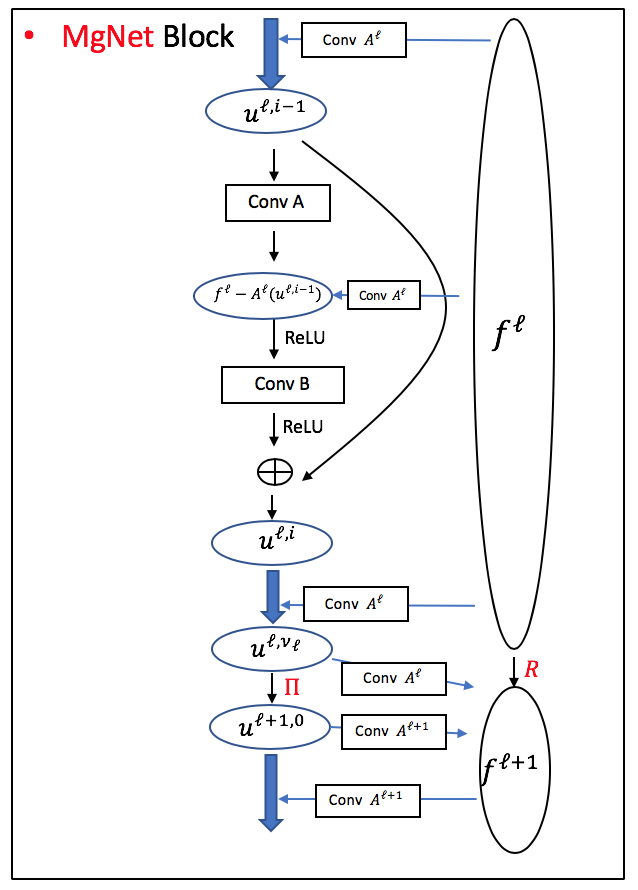
\includegraphics[width=.4\textwidth]{MgNet_3} 
	\end{center}
	\caption{Structure of MgNet}
	\label{fig:mgnet}
\end{figure}

The first property of MgNet is that it recovers the multigrid methods.
Despite of the simplicity look of Algorithm \ref{alg:mgnet}, there
are rich mathematical structures and variants which we will briefly discuss below.

\subsection{Initialization: feature space channels}
Initially for $\ell=1$,  we take $m_1 = m$ and $n_1 = n$ and we may define the linear mapping 
\begin{equation}
\label{eq:6}
\theta: \mathbb R^{c \times m\times n }
\mapsto \mathbb R^{c_1 \times m_1\times n_1 },
\end{equation}
to obtain $f^{1} = \theta(f)$ with $c$ %given in \eqref{data-c} 
changed to the channel of the initial
data space to $c_1$.   Usually
\begin{equation}
\label{cc}
c_1\ge c.  
\end{equation}
One possibility is that we choose $c_1=c$.  In this case, we choose
$\theta$ to be identity.   But in general, we may need to choose $c_1\gg
c$. One possible advantage of preprocessing the RGB ($c=3$) to 
different color spaces is that we can better choose what kind of
features the CNN can detect, and under what 
conditions those detections will be invariant.

One possibility of understanding and modifying this step 
is to decompose the data $f$ into a number of more
specialized data
\begin{equation}
\label{decomp-f}
f=\sum_{k=1}^{c_1}\xi_kf^1_k  =\xi^Tf^1.
\end{equation}
We may use some knowledge from image processing or physics to
design a procedure to obtain the right decomposition of
\eqref{decomp-f}, or we can just train it. 
Conceivably, we may view $f^{1} = \theta(f)$ as a special approximation solution of
\eqref{decomp-f} with the same sparsity pattern to $\xi$. 

\subsection{Extracted units: $u^{\ell}$ and channels}
The first new feature and the main new ingredient 
in the proposed neural network is the introduction 
of feature variables  $u^{\ell}$ in \eqref{u-ell}, which will be known
as the extracted units. 

We emphasize that the extracted-units $u^\ell$ and the data $f^\ell$ can have
different numbers of channels:\
\begin{equation}
\label{uf-channels}
u^\ell\in \mathbb{R}^{c_{u,\ell}\times m_\ell\times n_\ell  }, \quad
f^\ell\in \mathbb{R}^{c_{f,\ell} \times m_\ell\times n_\ell }
\end{equation}
One possibility is that the number of channels for both $u$ and $f$ remain
unchanged in different grids:  
\begin{equation}
\label{cfl}
c_{f,\ell}=c_f, \quad \ell=1:J,   
\end{equation}
and 
\begin{equation}
\label{ufl}
c_{u,\ell}=c_{u}, \quad \ell=1:J.   
\end{equation}
Both $c_f$ and $c_{u}$ are two super-parameters that need to be tuned, 
and we may even take $c_u = c_f$.

\subsection{Poolings: $\Pi_{\ell+1}^\ell$ and $R_{\ell+1}^\ell$}
The pooling $\Pi_{\ell+1}^\ell$ in \eqref{interpolation} and
$R_{\ell+1}^\ell$ in \eqref{restrict-f} are in general different.
They can be trained in general, but they may be a priori chosen.

There are many different possibilities to choose $\Pi_{\ell+1}^\ell$. 
The simplest choice of $\Pi_{\ell+1}^\ell$ is 
\begin{equation}
\label{eq:8}
\Pi_{\ell+1}^\ell=0.
\end{equation}
A more sophisticated choice can be obtained by considering an
interpolation from fine grid to coarse (that, for example preserves linear function
locally).  Namely
\begin{equation}
\label{Pi}
\Pi_{\ell+1}^\ell=\bar\Pi_{\ell+1}^\ell \otimes I_{c_\ell\times c_\ell} 
\end{equation}
with $\bar\Pi_{\ell+1}^\ell$ given in finite element methods.



\subsection{Data-feature mapping: $A^{\ell}$}
The second new feature of MgNet is that this data-feature mapping
only depends on the grid ${\cal T}_\ell$, and it does not depend on layers
within the same grid.  This amounts to a significant saving of the number of
parameters.  In comparison, the existing CNN, such as pre-act ResNet, can be
interpreted as a network related to the case that $A^{\ell}$ is
replaced by $A^{\ell, i}$, namely
\begin{equation}\label{u-resnet}
u^{\ell,i} = u^{\ell,i-1} + \sigma \circ B^{\ell,i} \ast \sigma (f^\ell -  A^{\ell,i} \ast u^{\ell,i-1}).
\end{equation}

The underlying convolution kernels can be different on different grids and they can
all be trained.


\subsection{Feature extractors: $\sigma \circ B^{\ell,i} \ast \sigma$}
Here we adopt the feature extractor as:
\begin{equation}
\label{extractor-ell}
\sigma\circ B^{\ell,i}\ast\sigma.
\end{equation}

Other than the level dependent extractors, the following 
different strategies can be used
\begin{description}
	\item[Constant Extractors]: $B^{\ell,i}=B^{\ell}$ for   $i=1:\nu_\ell$
	\item[Scaled Extractors]:$B^{\ell,i}=\alpha_iB^{\ell}$ for   $i=1:\nu_\ell$
	\item[Variable Extractors]: $B^{\ell,i}$
\end{description}



This brief framework gives us the basic principle on designing 
a CNN models for classification. All models are seen as the special
choice of data-feature mapping $A^\ell$, feature extractors $B^{\ell,i}$ 
and the pooling operators $\Pi_{\ell+1}^\ell$ with $R_{\ell+1}^\ell$.



%%%%%%%%%%%%%%%%%%%%%%%%%%%%%%%%%%%%
%%%%%%%%%%%%%%%%%%%%%%%%%%%%%%%%%%%%
%%%%%%%%%%%%%%%%%%%%%%%%%%%%%%%%%%%%

\endinput
Similarly, we can consider about the back-slash cycle process:
\begin{breakablealgorithm}
	\caption{$u^J={\rm MgNet1}(f; J,\nu_1, \cdots, \nu_J; \nu'_1, \cdots, \nu'_J )$}
	\label{alg:mgnet1}
	\begin{algorithmic}
		\State 
		$$
		(\bar u^{1,0}, \bar u^1, f^1, \bar u^{2,0}, u^2, f^2,\cdots, \bar u^{J,0},\bar u^J, f^J) = \text{MgNet}(f; J,\nu_1, \cdots, \nu_J).
		$$
		%\State Define $\bar u^{\ell, 0 } = u^{\ell,0}$ for $\ell = 1:J$.
		\For{$\ell = J-1 : 1$}
		%		\State  and $u^{\ell,\nu_\ell'} = u^{\ell}$ then
		\begin{equation}
		%		\begin{aligned}
		u^{\ell,0} \leftarrow \bar u^{\ell} + R_{\ell}^{\ell+1} \ast_2^T (u^{\ell+1} - \bar u^{\ell+1,0}).
		%		\end{aligned}
		\end{equation}
		%				f^\ell &= f^\ell - A^\ell \bar u^{\ell,0}+ A^\ell  u^{\ell,0}. 
		\For{$i = 1:\nu'_\ell$}
		\State 
		\begin{equation}\label{mgnet}
		u^{\ell,i} \leftarrow u^{\ell,i-1} + (B^{\ell,i})'  ({f^\ell -  A^{\ell} \ast u^{\ell,i-1}}).
		\end{equation}
		\EndFor
		\State  
		$$
		u^{\ell} \leftarrow u^{\ell,\nu_\ell'} .
		$$
		\EndFor
		\State 
		$$
		(u^1,\cdots, u^{J-1}).
		$$
	\end{algorithmic}
\end{breakablealgorithm}
